\documentclass{article}

\usepackage{graphicx}
\usepackage{tikz}
\usepackage{tikzsymbols}
\usetikzlibrary{calc,patterns,shapes.geometric}
\pagestyle{empty}
\usepackage[margin=0pt]{geometry}
\geometry{papersize={14in,12in}}

\def\centerarc[#1](#2)(#3:#4:#5){\draw[#1] ($(#2)+({#5*cos(#3)},{#5*sin(#3)})$) arc (#3:#4:#5);}

\begin{document}
	\begin{figure}
		\centering
		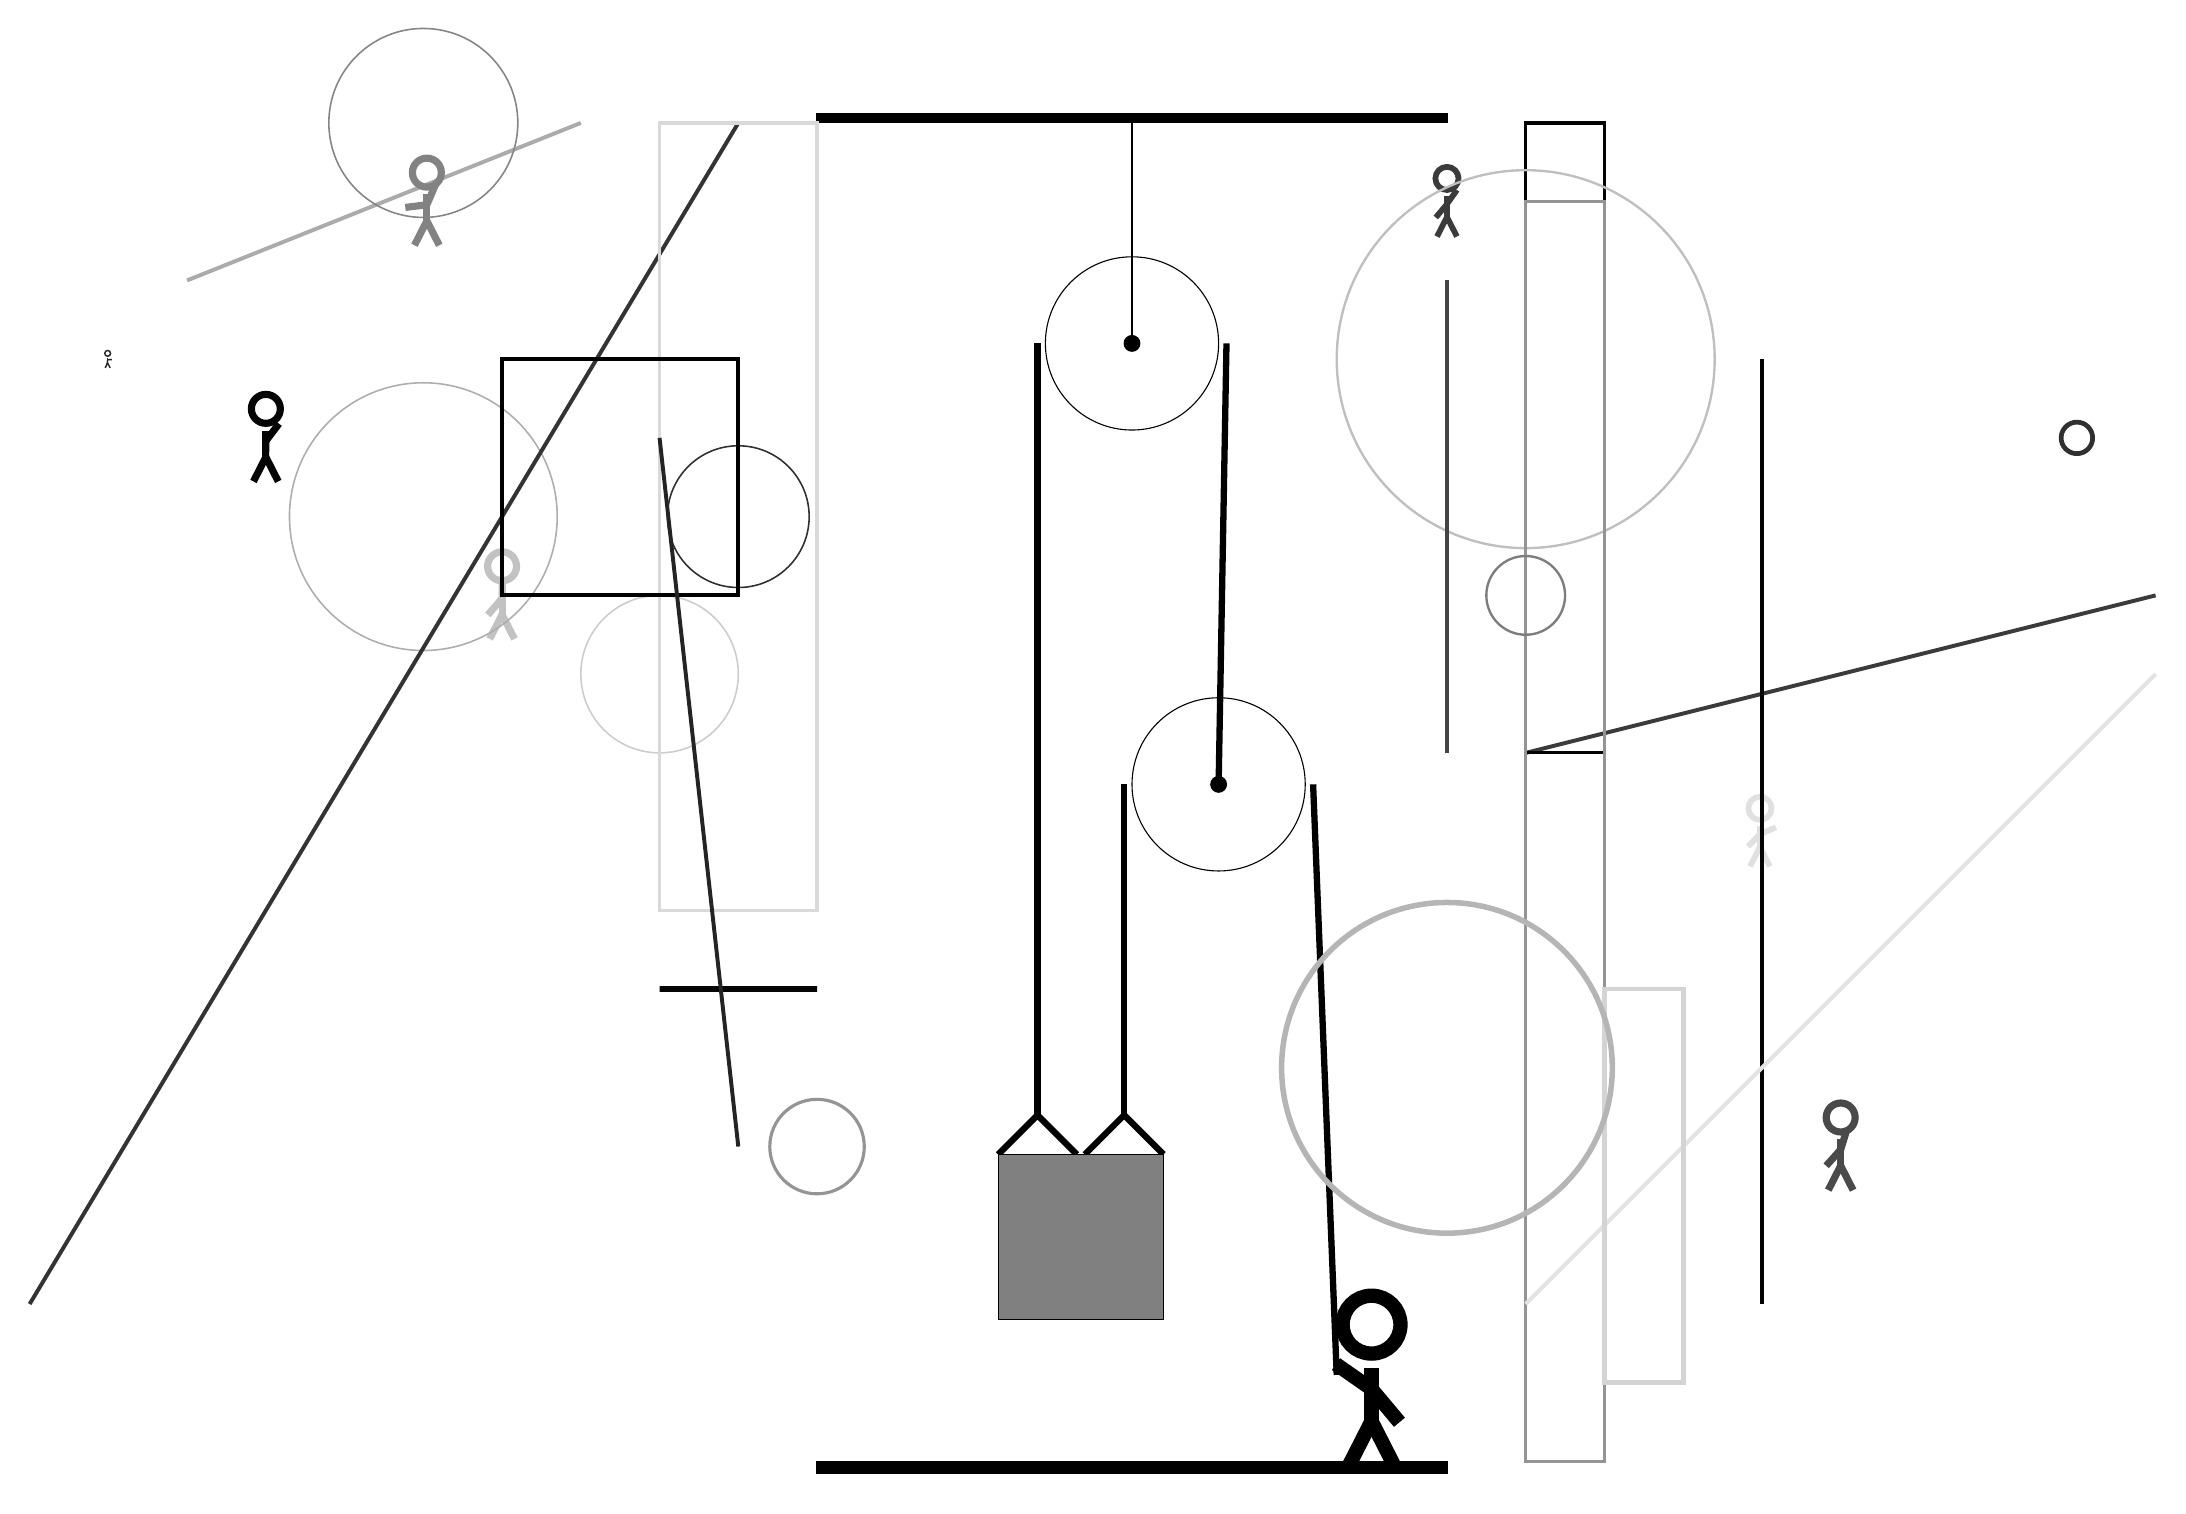
\begin{tikzpicture}
			%%%%% START %%%%%
			
			\draw[fill=black] (-2, 14) rectangle (6, 14.125);
			
			\draw (2, 11.2) circle (1.1);
			\draw[fill=black] (2, 11.2) circle (0.1);
			\draw[thick] (2, 11.2) -- (2, 14);
			
			\draw (3.1, 5.6) circle (1.1);
			\draw[fill=black] (3.1, 5.6) circle (0.1);
			
			\draw[line width = 0.8mm]  (0.3, 0.9) -- (0.8, 1.4) -- (1.3, 0.9);
			\draw[line width = 0.8mm]  (1.4, 0.9) -- (1.9, 1.4) -- (2.4, 0.9);
			\draw[fill=black!50] (0.3, 0.9) rectangle (2.4, -1.2);
			
			\draw[line width = 0.8mm] (0.8, 11.2) -- (0.8, 1.4);
			\centerarc[line width = 0.8mm](2, 11.2)(0:180:1.2000000000000002);
			\draw[line width = 0.8mm] (3.2, 11.2) -- (3.1, 5.6);
			\draw[line width = 0.8mm] (1.9, 5.6) -- (1.9, 1.4);
			\centerarc[line width = 0.8mm](3.1, 5.6)(0:180:1.2000000000000002);
			\draw[line width = 0.8mm] (4.3, 5.6) -- (4.6, -1.9);
			
			\node at (5, -2) {\Strichmaxerl[10][-35][-50]};
			
			\node[line width=0.5mm, color=black!24] at (-6, 8) {\Strichmaxerl[5][49][89]};
			
			\draw[line width=0.5mm, color=black!33](-5, 14) -- (-10, 12);
			\draw [line width=0.2mm, color=black!32](-7, 9) circle (1.7);
			\node[line width=0.7mm, color=black!12] at (10, 5) {\Strichmaxerl[4][46][23]};
			
			\draw[line width=0.5mm, color=black!77](7, 6) -- (15, 8);
			
			\draw[line width=0.4mm, color=black!99] (7, 6) rectangle (8, 14);
			\draw [line width=0.2mm, color=black!20](-4, 7) circle (1.0);
			\draw [line width=0.6mm, color=black!81](14, 10) circle (0.2);
			\draw[line width=0.5mm, color=black!99](10, 11) -- (10, -1);
			\draw [line width=0.2mm, color=black!81](-3, 9) circle (0.9);
			
			\draw[line width=0.5mm, color=black!80](-3, 14) -- (-12, -1);
			\node[line width=0.3mm, color=black!77] at (6, 13) {\Strichmaxerl[4][50][55]};
			\draw [line width=0.3mm, color=black!25](7, 11) circle (2.4);
			
			\draw [line width=0.2mm, color=black!48](-7, 14) circle (1.2);
			\draw[line width=0.4mm, color=black!42] (7, 13) rectangle (8, -3);
			\node[line width=0.7mm, color=black!49] at (-7, 13) {\Strichmaxerl[5][7][67]};
			\draw[line width=0.5mm, color=black!11](7, -1) -- (15, 7);
			\draw[line width=0.7mm, color=black!98] (-2, 3) rectangle (-4, 3);
			\draw[line width=0.6mm, color=black!17] (8, -2) rectangle (9, 3);
			\draw[line width=0.4mm, color=black!15] (-4, 4) rectangle (-2, 14);
			\node[line width=0.2mm, color=black!71] at (11, 1) {\Strichmaxerl[5][48][73]};
			
			\node[line width=0.6mm, color=black!98] at (-9, 10) {\Strichmaxerl[5][89][53]};
			\node[line width=0.7mm, color=black!86] at (-11, 11) {\Strichmaxerl[1][83][3]};
			\draw[line width=0.5mm, color=black!73](6, 12) -- (6, 6);
			\draw[line width=0.5mm, color=black!100] (-3, 8) rectangle (-6, 11);
			
			\draw[line width=0.5mm, color=black!86](-3, 1) -- (-4, 10);
			
			\draw [line width=0.7mm, color=black!29](6, 2) circle (2.1);
			\draw [line width=0.3mm, color=black!51](7, 8) circle (0.5);
			\draw [line width=0.4mm, color=black!42](-2, 1) circle (0.6);
			
			
			\draw[fill=black] (-2, -3) rectangle (6, -3.15);
			
			%%%%% END %%%%%
		\end{tikzpicture}
	\end{figure}	
\end{document}